\section{From a policy to a tree}
\begin{algorithm}[t]
    \KwData{Deterministic partially observable policy $\pi_{po}$ for IBMDP $\mathcal{M}_{IB}\equiv \langle S \times O,A \cup A_{info}, (R, \zeta), (T_{info}, T, T_0)\rangle$ and IBMDP observation $\boldsymbol{o}=(L'_1, U'_1, \dots, L'_p, U'_p)$}
    \KwResult{Decision tree policy $\pi_{\mathcal{T}}$ for MDP $\mathcal{M}\equiv\langle S, A, R, T, T_0\rangle$}
    
    \SetKwProg{Fn}{Function}{:}{}
    \SetKwFunction{SubtreeFromPolicy}{Subtree\_From\_Policy}
    
    \Fn{\SubtreeFromPolicy{$\boldsymbol{o}, \pi_{po}$}}{
        $a \leftarrow \pi_{po}(\boldsymbol{o})$ \\
        \If{$a$ is a downstream action}{
            \Return Leaf\_Node(action: $a$)
        }
        \Else{
            $\langle i, v\rangle \leftarrow a$\\
            $\boldsymbol{o}_L \leftarrow \boldsymbol{o}; \quad \boldsymbol{o}_R \leftarrow \boldsymbol{o}$ \\
                         $\boldsymbol{o}_L \leftarrow (L'_1, U'_1, \dots, L'_j, v, \dots, L'_p, U'_p); \quad \boldsymbol{o}_R \leftarrow (L'_1, U'_1, \dots, v, U'_j, \dots, L'_p, U'_p)$ \\
            $child_L \leftarrow$ Subtree\_From\_Policy$(\boldsymbol{o}_L, \pi_{po})$ \\
            $child_R \leftarrow$ Subtree\_From\_Policy$(\boldsymbol{o}_R, \pi_{po})$ \\
            \Return Internal\_Node(feature: $i$, value: $v$, children: $(child_L, child_R)$)
        }
    }
    \caption{Extract a decision tree policy (algorithm 1 from~\citet{topin2021iterative})}\label{alg:extract-tree}
\end{algorithm}

\section{Imitation learning: a baseline for indirect decision tree policy learning}\label{sec:imit}
In this section we present decision tree policies of this manuscript obtained using Dagger or VIPER~\cite{viper,pirl} after learning an expert Q-function for the grid world MDP.
Recall the optimal policies for the grid world, taking the green actions in each state in figure~\ref{fig:mdp-dt}. 
Among the optimal policies, the ones that go left or up in the goal state can be problematic for imitation learning algorithms.
Indeed, we know that for this grid world MDP there exists decision tree policies with a very good interpretability-performance trade-off: depth-1 decision trees that are optimal w.r.t. the RL objective.
One could even say that those trees have the \textit{optimal} interpretability-performance trade-off because they are the shortest trees that are optimal w.r.t. the RL objective.

In figure~\ref{fig:trees-intro}, we present a depth-1 decision tree policy that is optimal w.r.t. the RL objective and a depth-1 tree that is sub-optimal.
The other optimal depth-1 tree is to go right when $y\leq 1$ and down otherwise.

Now a fair question is: can Dagger or VIPER learn such an optimal depth-1 tree given access to an expert optimal policy from figure~\ref{fig:mdp-dt}?

We start by running the standard Q-learning algorithm with $\epsilon=0.3$, $\alpha=0.1$ over 10,000 time steps.
While for Q-learning, Sutton and Barto break ties by index value in their book~\cite{sutton} (the greedy action is the $\operatorname{argmax}$ action with smallest index), we show that the choice of tie-breaking greatly influences the performance of subsequent imitation learning algorithms.
Indeed, depending on how actions are ordered in practice, Q-learning may be biased toward some optimal policies rather than others.
While this does not matter for one who just wants to find an optimal policy, in our example of finding the optimal depth-1 decision tree policy, it matters \textit{a lot}.

In the left plot of figure~\ref{fig:ql-il}, we see that Q-learning, independently of how ties are broken, consistently converges to an optimal policy over 100 runs (random seeds).
However, in the right plot of figure~\ref{fig:ql-il}, where we plot the proportion over 100 runs of optimal decision trees returned by Dagger or VIPER at different stages of Q-learning, we observe that imitating the optimal policy obtained by breaking ties at random consistently yields more optimal trees than breaking ties by indices.
What actually happens is that the most likely output of Q-learning when ties are broken by indices is the optimal policy that goes left in the goal state,
which cannot be perfectly represented by a depth-1 decision tree, because there are three different actions taken and a binary tree of depth $D=1$ can only map to $2^D=2$ labels.

This short experiment shows that imitation learning approaches can sometimes be very bad at learning decision tree policies with good interpretability-performance trade-offs for very simple MDPs. 
Despite VIPER almost always finding the optimal depth-1 decision tree policy in terms of the RL objective when ties are broken at random, we have shed light on the sub-optimality of indirect approaches such as imitation learning.
This motivates the study of direct approaches to directly search for policies with good interpretability-performance trade-offs with respect to the original RL objective.

\begin{figure}
    \centering
    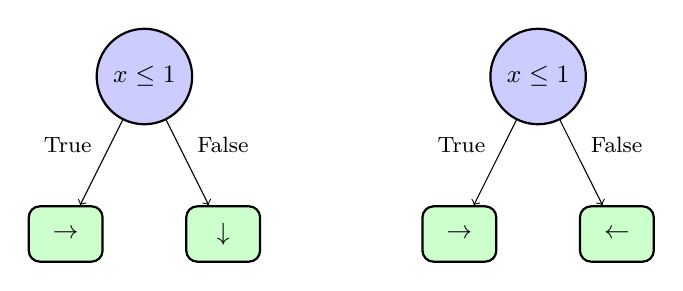
\begin{tikzpicture}[
        decision/.style={circle, draw, thick, fill=blue!20, text width=2.5em, text centered, minimum height=2.5em, font=\small},
        leaf/.style={rectangle, draw, thick, fill=green!20, text width=2em, text centered, rounded corners, minimum height=2em, font=\small},
        edge_label/.style={font=\footnotesize, midway}
    ]
        % Tree 4: if x <= 0.5 move right else move left
        \node[decision] (tree4_root) at (10,2) {$x \leq 1$};
        \node[leaf] (tree4_right) at (9,0) {$\rightarrow$};
        \node[leaf] (tree4_left) at (11,0) {$\leftarrow$};
        \draw[->] (tree4_root) -- (tree4_right) node[edge_label, above left] {True};
        \draw[->] (tree4_root) -- (tree4_left) node[edge_label, above right] {False};
        \tikzstyle{grid}=[draw, thick, fill=gray!10]


        % Tree 4: if x <= 0.5 move right else move left
        \node[decision] (tree5_root) at (5,2) {$x \leq 1$};
        \node[leaf] (tree5_right) at (4,0) {$\rightarrow$};
        \node[leaf] (tree5_left) at (6,0) {$\downarrow$};
        \draw[->] (tree5_root) -- (tree5_right) node[edge_label, above left] {True};
        \draw[->] (tree5_root) -- (tree5_left) node[edge_label, above right] {False};
        \tikzstyle{grid}=[draw, thick, fill=gray!10]

    \end{tikzpicture}
    \caption{Left, an optimal depth-1 decision tree policy for the grid world MDP from figure~\ref{fig:mdp-dt}. On the right, a sub-optimal depth-1 decision tree policy.}\label{fig:trees-intro}
    \end{figure}

\begin{figure}
    \centering
    \includegraphics[width=1\textwidth]{../images/images_part1/base_mdp.pdf}
    \caption{Left, sample complexity curve of Q-learning with default hyperparameters on the $2\times 2$ grid world MDP over 100 random seeds. Right, performance of indirect interpretable methods when imitating the greedy policy with a tree at different Q-learning stages.}\label{fig:ql-il}
\end{figure}

\section{Reproducing ``Iterative Bounding MDPs: Learning Interpretable Policies via Non-Interpretable Methods''}\label{sec:reprod}
We attempt to reproduce the results from~\cite{topin2021iterative} in which authors compare direct and indirect learning of decision tree policies of depth at most 2 for the CartPole MDP~\cite{cartpole}.
In the original paper, the authors find that both direct and indirect learning yields decision tree policies with similar RL objective values (definition~\ref{def:mdp-obj}) for the CartPole.
On the other hand, we find that, imitation learning, despite not directly optimizing the RL objective for CartPole, outperforms deep RL which directly optimizes a trade-off of the standard RL objective and interpretability.

Authors of~\citet{topin2021iterative} use two deep reinforcement learning baselines to which they apply some modifications in order to learn memoryless policies.
Authors modify the standard DQN~\cite{DQN} to return a memoryless policy. The trained $Q$-function is approximated with a neural network $O\rightarrow \mathbb{R}^{|A\cup A_{info}|}$ rather than $S\times O\rightarrow \mathbb{R}^{|A\cup A_{info}|}$.
In this modified DQN, the temporal difference error target for the $Q$-function $O\rightarrow A\cup A_{info}$ is approximated by a neural network $S\times O\rightarrow A\cup A_{info}$ that is in turn trained by bootstrapping the temporal difference error with itself.
We present the modifications in algorithm~\ref{alg:mod-dqn}.
Similar modifications are applied to the standard PPO~\cite{ppo} that we present in the appendix (algorithm \ref{alg:mod-ppo}). In the modified PPO, neural network policy $O\rightarrow A\cup A_{info}$ is trained using a neural network value function $S\times O\rightarrow A\cup A_{info}$ as a critic.

Those two variants of DQN and PPO have first been introduced in \cite{pinto} for robotic tasks with partially observable components, under the name ``asymmetric'' actor-critic. 
Asymmetric RL algorithms that have policy and value estimates using different information from a POMDP~\cite{POMDP,chap2} were later studied theoretically to solve POMDPs in Baisero's work~\cite{baisero-dqn,baisero-ppo}.
The connections from Deep RL in IBMDPs for objective is absent from \cite{topin2021iterative} and we defer their connections to direct interpretable reinforcement learning to the next chapter as our primary goal is to reproduce \cite{topin2021iterative} \textit{as is}.
Next, we present the precise experimental setup we use to reproduce~\cite{topin2021iterative} in order to study direct deep reinforcement learning of decision tree policies for the CartPole MDP.

\subsection{IBMDP formulation}\label{sec:ibmdp-paper}
Given a base MDP $\mathcal{M}\equiv\langle S, A, R, T, T_0\rangle$ (cf. definition~\ref{def:mdp}), in order to define an IBMDP $\mathcal{M}_{IB}\langle S\times O, A\cup A_{info}, (R, \zeta),( T, T_0, T_{info})\rangle$ (cf. definition~\ref{def:ibmdp}), the user needs to provide the set of information gathering actions $A_{info}$ and the reward $\zeta$ for taking those.
Authors of~\citer{topin2021iterative} propose to parametrize the set of IGAs with $j \times q$ actions $\langle j, v_k \rangle$ with $v_k$ depending on the current observation $\boldsymbol{o}_t=(L'_1, U'_1, \dots, L'_j, U'_j, \dots, L'_p, U'_p)$: $v_k = \frac{k(U'_j - L'_j)}{q+1}$.
This parametric IGAs space keeps the discrete IBMDP action space at a reasonable size while providing a learning algorithm with varied IGAs to try.

For example, if we define an IBMDP with $q=3$ for the grid world from figure~\ref{fig:mdp-dt}, the grid world action space is augmented with six IGAs. 
At $t=0$, recall that $\boldsymbol{o}_0=(0, 2, 0, 2)$, so if an IGA is taken, e.g. $\langle 2, v_2\rangle$, the effective IGA is $\langle j, v_2=\frac{k(2-0)}{3+1}\rangle = \langle 1, 2 \rangle$ which in turn effectively corresponds to an internal decision tree node $y \leq 1$.
If the current state $y$-feature value is $0.5$, then the next observation at $t=1$ is $\boldsymbol{o}_1=(0, 2, 0, 1)$. At $t=2$ if $a_t=\langle 2, v_2 \rangle$ again, it would be effectively $\langle j, v_2=\frac{k(1-0)}{3+1}\rangle = \langle 2, 0.5 \rangle$. 
This would give the next observation at $t=2$ $\boldsymbol{o}_2=(0, 2, 0, 0.5)$ and so on. 

Furthermore, author propose to regularize the learned decision tree policy with a maximum depth parameter $D$.
Unfortunately, the authors did not describe how they implemented the depth control in their work, hence we have to try different approaches to reproduce their results.

To control the tree depth during learning in the IBMDP, we can either give negative reward for taking $D$ IGAs in a row, or terminate the trajectory.
In practice, we could also have a state-dependent action space such that taking an IGA is not allowed after taking $D$ IGAs in a row.
The latter approach--sometimes called action masking--is not compatible with the definition of an MDP (cf. definition~\ref{def:mdp}) in which all actions are available in all states. 
To apply the penalization approaches, one can extend the MDP states to keep track of the current tree depth.
Similarly, the termination approach requires a transition function that depends on the current tree depth.

We actually find that when $q+1$, the parameter that defines threshold values in decision tree policy nodes (cf. definition~\ref{def:ibmdp}), is a prime number, then as a direct consequence of the \textit{Chinese Remainder Theorem}\footnote{\url{https://en.wikipedia.org/wiki/Chinese_remainder_theorem}}, the current tree depth is directly encoded in the current observation $\boldsymbol{o}_t$. 
Hence, when $q+1$ is prime, we can control the depth through either transitions or rewards without tracking the tree depth.
We use the exact same downstream MDP and associated IBMDPs for our experiments as~\cite{topin2021iterative} except when mentioned otherwise.

\paragraph{downstream MDP} The task at hand is to optimize the RL objective (definition~\ref{def:mdp-obj}) with a decision tree policy for the CartPole MDP~\cite{cartpole}.
At each time step a learning algorithm observes the cart's position and velocity and the pole's angle and angular velocity, and can take action to push the CartPole left or right.
While the CartPole is roughly balanced, i.e., while the cart's angle remains in some fixed range, the agent gets a positive reward.
If the CartPole is out of balance, the MDP transitions to an absorbing terminal state and gets 0 reward forever.
Like in~\cite{topin2021iterative}, we use the gymnasium \texttt{CartPole-v0} implementation~\cite{gymnasium} of the CartPole MDP in which trajectories are truncated after 200 timesteps making the maximum cumulative reward, i.e. the optimal value of the RL objective when $\gamma=1$, to be 200.
The state features of the CartPole MDP are in $[-2, 2] \times [-2, 2] \times [-0.14, 0.14] \times [-1.4, 1.4]$.

\paragraph{IBMDP} Authors define the associated IBMDP (definition~\ref{def:ibmdp}) with $\zeta=-0.01$ and 4 information gathering actions.
In addition to the original IBMDP paper, we also try $\zeta=0.01$ and 3 information gathering actions.
We use the same discount factor as the authors: $\gamma=1$.
We try two different approaches to limit the depth of decision tree policies to be at most 2: terminating trajectories if the agent takes too many information gathering actions in a row or simply giving a reward of $-1$ to the agent every time it takes an information gathering action past the depth limit.
In practice, we could have tried an action masking approach, i.e. having a state dependent-action set, but we want to abide to the MDP formalism in order to properly understand direct interpretable approaches.
We will also try IBMDPs where we do not limit the maximum depth for completeness.

\begin{table}[H]
    \centering
    \caption{IBMDP hyperparameters. We try 12 different IBMDPs. In green we highlight the hyperparameters from the original paper and in red we highlight the hyperparameter names for which author do not give information.}\label{tab:ibmdp-params}
    \begin{tabular}{ll}
    \toprule
    \textbf{Hyperparameter} & \textbf{Values}\\
    \midrule
    Discount factor $\gamma$ & \textcolor{green}{1} \\
    Information gathering actions parameter $q$ & 2, \textcolor{green}{3} \\
    Information gathering actions rewards $\zeta$ & \textcolor{green}{-0.01}, 0.01 \\
    \textcolor{red}{Depth control} & Done signal, negative reward, none \\ 
    \bottomrule
    \end{tabular}
    \end{table}


\begin{table}[H]
    \centering
    \caption{(Modified) DQN trained on $10^6$ timesteps. This gives four different instantiation of (modified) DQN. Hyperparameters not mentioned are stable-baselines3 default. In green we highlight the hyperparameters from the original paper and in red we highlight the hyperparameter names for which author do not give information.}\label{tab:ibmdp-rl1}
    \begin{tabular}{ll}
    \toprule
    \textbf{Hyperparameter} & \textbf{Values}\\
    \midrule
    Buffer size & \textcolor{green}{$10^6$} \\
    Random transitions before learning & \textcolor{green}{$10^5$} \\
    Epsilon start & 0.9, \textcolor{green}{0.5} \\
    Epsilon end & \textcolor{green}{0.05} \\
    Exploration fraction & \textcolor{green}{0.1} \\
    Optimizer & \textcolor{green}{RMSprop ($\alpha = 0.95$)}\\
    Learning rate & \textcolor{green}{$2.5\times10^{-4}$}\\
    Networks architectures & \textcolor{green}{[128, 128]}\\
    \textcolor{red}{Networks activation} & $\operatorname{tanh()}$, $\operatorname{relu()}$\\
    \bottomrule
    \end{tabular}
    \end{table}

\begin{table}[H]
    \centering
    \caption{(Modified) PPO trained on $4\times10^6$ timesteps. This gives two different instantiation of (modified) PPO. Hyperparameters not mentioned are stable-baselines3 default. In green we highlight the hyperparameters from the original paper and in red we highlight the hyperparameter names for which author do not give information.}\label{tab:ibmdp-rl2}
    \begin{tabular}{ll}
    \toprule
    \textbf{Hyperparameter} & \textbf{Values}\\
    \midrule
    Steps between each policy gradient steps & \textcolor{green}{512} \\
    Number of minibatch for policy gradient updates & \textcolor{green}{4} \\
    Networks architectures & \textcolor{green}{[64, 64]}\\
    \textcolor{red}{Networks activations} & $\operatorname{tanh()}$, $\operatorname{relu()}$\\
    \bottomrule
    \end{tabular}
    \end{table}


In tables~\ref{tab:mod-dqn} and~\ref{tab:mod-ppo} we report the top-5 hyperparameters for Modified RL baselines when learning partially observable IBMDP policies in terms of extracted decision tree policies performances in the CartPole MDP.
\begin{table}
    \centering
    \caption{Top 5 hyperparameter configurations for modified DQN + IBMDP, bold font represent the original paper hyperparameters.}\label{tab:mod-dqn}
    \label{tab:top5_results}
    \begin{tabular}{ccccccS}
    \toprule
    Rank & $q$ & Depth control & Activation & Exploration & $\zeta$ & {Mean Final Performance} \\
    \midrule
    1 & 3 & termination & $\operatorname{tanh}$ & 0.9 & 0.01 & 53 \\
    2 & 2 & termination & $\operatorname{tanh}$ & 0.5 & -0.01 & 24 \\
    \textbf{3} & \textbf{3} & \textbf{termination} & $\operatorname{tanh}$ & \textbf{0.5} & \textbf{-0.01} & \textbf{24} \\
    4 & 2 & termination & $\operatorname{tanh}$ & 0.5 & 0.01 & 23 \\
    5 & 2 & termination & $\operatorname{tanh}$ & 0.9 & -0.01 & 22 \\
    \bottomrule
    \end{tabular}
    \end{table}

    \begin{table}
        \centering
        \caption{Top 5 hyperparameter configurations for modified PPO + IBMDP, bold font represent the original paper hyperparameters.}\label{tab:mod-ppo}
        \label{tab:top5_ppo_results}
        \begin{tabular}{cccccS}
        \toprule
        Rank & $q$ & Depth Control & Activation & $\zeta$ & {Mean Final Performance} \\
        \midrule
        1 & 3 & reward & $\operatorname{relu}$ & 0.01 & 139 \\
        2 & 3 & termination & $\operatorname{relu}$ & 0.01 & 132 \\
        \textbf{3} & \textbf{3} & \textbf{reward} & $\operatorname{tanh}$ & \textbf{-0.01} & \textbf{119} \\
        4 & 3 & reward & $\operatorname{relu}$ & -0.01 & 117 \\
        5 & 3 & reward & $\operatorname{tanh}$ & 0.01 & 116 \\
        \bottomrule
        \end{tabular}
        \end{table}


\begin{algorithm}
    \KwData{IBMDP $\mathcal{M}_{IB}\langle S\times O, A\cup A_{info}, (R, \zeta),( T, T_0, T_{info})\rangle$, learning rate $\alpha$, exploration rate $\epsilon$, partially observable Q-network parameters $\theta$, Q-network parameters $\phi$, replay buffer $\mathcal{B}$, update frequency $C$}
    \KwResult{deterministic memoryless policy $\pi_{po}$}
    Initialize partially observable Q-network parameters $\theta$\\
    \textcolor{teal}{Initialize Q-network parameters $\phi$ and target network parameters $\phi^- = \phi$} \\

    Initialize replay buffer $\mathcal{B} = \emptyset$ \\
    \For{each episode}{
        Initialize downstream state features $\boldsymbol{s}_0 \sim T_0$ \\
        Initialize observation $\boldsymbol{o}_0 = (L_1, U_1, \dots, L_p, U_p)$ \\

        \For{each step $t$}{
            Choose action $a_t$ using $\epsilon$-greedy: $a_t = \operatorname{argmax}_a Q_\theta(\boldsymbol{o}_t,a)$ with prob. $1-\epsilon$ \\
            Take action $a_t$, observe $r_t$ \\
            Store transition $(\boldsymbol{s}_t, \boldsymbol{o}_t, a_t, r_t, \boldsymbol{s}_{t+1})$ in $\mathcal{B}$ \\
            Sample random batch $(\boldsymbol{s}_i, \boldsymbol{o}_i, a_i, r_i, \boldsymbol{s}_{i+1}) \sim \mathcal{B}$ \\
            $a' = \underset{a}{\operatorname{argmax}} Q_{\theta}(\boldsymbol{o}_i, a)$ \\
            \textcolor{teal}{$y_i = r_i + \gamma Q_{\phi^-}(\boldsymbol{s}_{i+1}, a')$} \Comment{// Compute target}
            $\phi \leftarrow \phi - \alpha \nabla_\phi (Q_\phi(\boldsymbol{s}_i, a_i) - y_i)^2$ \Comment{// Update Q-network}
            \textcolor{teal}{$\theta \leftarrow \theta - \alpha \nabla_\theta (Q_\theta(\boldsymbol{o}_i, a_i) - y_i)^2$} \Comment{// Update partially observable Q-network}

            \If{$t \bmod C = 0$}{
                $\theta^- \leftarrow \theta$ \Comment{// Update target network}
            }
            $\boldsymbol{s}_t \leftarrow \boldsymbol{s}_{t+1}$ \\
            $\boldsymbol{o}_t \leftarrow \boldsymbol{o}_{t+1}$ \\
        }
    }
    $\pi_{po}(\boldsymbol{o}) = \operatorname{argmax}_a Q_\theta(\boldsymbol{o},a)$ \Comment{// Extract greedy policy}
    \caption{Modified Deep Q-Network. We highlight in green the changes to the standard DQN~\cite{dqn}.}\label{alg:mod-dqn}
\end{algorithm}

\begin{algorithm}
    \KwData{IBMDP $\mathcal{M}_{IB}\langle S\times O, A\cup A_{info}, (R, \zeta),( T, T_0, T_{info})\rangle$, learning rate $\alpha$, policy parameters $\theta$, clipping parameter $\epsilon$, value function parameters $\phi$}
    \KwResult{Memoryless stochastic policy $\pi_{po_\theta}$}
    Initialize policy parameters $\theta$ and value function parameters $\phi$ \\
    \For{each episode}{
        Generate trajectory $\tau = (\boldsymbol{s}_0, \boldsymbol{o}_0, a_0, r_0, \boldsymbol{s}_1, \boldsymbol{o}_1, a_1, r_1, \ldots)$ following $\pi_\theta$ \\
        \For{each timestep $t$ in trajectory}{
            $G_t \leftarrow \sum_{k=t}^{T} \gamma^{k-t} r_k$ \Comment{// Compute return}
            $A_t \leftarrow G_t - V_\phi(\boldsymbol{s}_t)$ \Comment{// Compute advantage}
            $r_t(\theta) \leftarrow \frac{\pi_{po_\theta}(a_t|\boldsymbol{o}_t)}{\pi_{po_\theta}_{old}(a_t|\boldsymbol{o}_t)}$ \Comment{// Compute probability ratio}
            $L^{CLIP}_t \leftarrow \min(r_t(\theta) A_t, \text{clip}(r_t(\theta), 1-\epsilon, 1+\epsilon) A_t)$ \Comment{// Clipped objective}
            $\theta \leftarrow \theta + \alpha \nabla_\theta L^{CLIP}_t$ \Comment{// Policy update}
            $\phi \leftarrow \phi + \alpha \nabla_\phi (G_t - V_\phi(\boldsymbol{s}_t))^2$ \Comment{// Value function update}
        }
        $\theta_{old} \leftarrow \theta$ \Comment{// Update old policy}
    }
    \caption{Modified Proximal Policy Optimization}\label{alg:mod-ppo}
\end{algorithm}

\subsection{Experimental setup}

\paragraph{Modified DQN and Modified PPO} as mentioned above, the authors use the modified version of DQN from algorithm~\ref{alg:mod-dqn}.
We use the exact same hyperparameters for modified DQN as the authors when possible. 
We use the same layers width (128) and number of hidden layers (2), the same exploration strategy ($\epsilon$-greedy with linearly decreasing value $\epsilon$ between 0.5 and 0.05 during the first 10\% of the training),
the same replay buffer size ($10^6$) and the same number of transitions to be collected randomly before doing value updates ($10^5$).
We also try to use more exploration during training (change the initial $\epsilon$ value to 0.9).
We use the same optimizer (RMSprop with hyperparameter 0.95 and learning rate $2.5 \times 10^{-4}$) to update the $Q$-networks.
Authors did not share which DQN implementation they used so we use the stable-baselines3 one~\cite{stable-baselines3}\footnote{We are cleaning our source code and will open source it as soon as possible}.
Authors did not share which activation functions they used so we try both $\operatorname{tanh}$ and $\operatorname{relu}$. 
For the modified PPO algorithm (algorithm~\ref{alg:mod-ppo}), we can exactly match the authors hyperparameters since they use the open source stable-baselines3 implementation of PPO.
We match training budgets: we train modified DQN on 1 million timesteps and modified PPO on 4 million timesteps.

\paragraph{DQN and PPO} We also benchmark the standard DQN and PPO when learning standard Markovian IBMDP policies $\pi:S\times O\rightarrow A\cup A_{info}$ and when learning standard $\pi:S\rightarrow A$ policies directly in the CartPole MDP.
We summarize hyperparameters for the IBMDP and for the learning algorithms in appendices~\ref{tab:ibmdp-params}, \ref{tab:ibmdp-rl1} and \ref{tab:ibmdp-rl2}.

\paragraph{Indirect methods} We also compare modified RL algorithm to imitation learning.
To do so, we use VIPER or Dagger to imitate greedy neural network policies obtained with standard DQN learning directly on CartPole.
We use Dagger to imitate neural network policies obtained with the standard PPO learning directly on CartPole. 
For each indirect method, we imitate the neural network experts by fitting decision trees on 10000 expert transitions using the CART~\cite{breiman1984classification} implementation from scikit-learn~\cite{scikit-learn} with default hyperparameters and maximum depth of 2 like in ~\cite{topin2021iterative}.
    
\subsubsection{Metrics}
The key metric of this section is performance when controlling the CartPole, i.e, the average \textit{undiscounted} cumulative reward of a policy on 100 trajectories (RL objective with $\gamma=1$).
For modified RL algorithms that learn a memoryless policy (or $Q$-function) in an IBMDP, we periodically extract the policy (or $Q$-function) and use algorithm~\ref{alg:extract-tree} to extract a decision tree for the CartPole MDP. 
We then evaluate the tree on 100 independent trajectories in the MDP and report the mean undiscounted cumulative reward.
For RL applied to IBMDPs, since we can't deploy learned policies directly to the downstream MDP as the state dimensions mismatch--such policies are $S\times O\rightarrow A \cup A_{info}$ but the MDP states are in $S$--we periodically evaluate those IBMDP policies in a copy of the IBMDP in which we fix $\zeta=0$ ensuring that the copied IBMDP undiscounted cumulative rewards only account rewards from the CartPole MDP (non-zero rewards in the IBMDP only occur when a reward from the downstream MDP is given, i.e. when $a_t\in A$ in the IBMDP (definition~\ref{def:ibmdp})).
Similarly, we do 100 trajectories of the extracted policies in the copied IBMDP and report the average undiscounted cumulative reward.
For RL applied directly to the downstream MDP we can just periodically extract the learned policies and evaluate them on 100 CartPole trajectories.

Since imitation learning baselines train offline, i.e, on a fixed dataset, their performances cannot directly be reported on the same axis as RL baselines.
For that reason, during the training of a standard RL baseline, we periodically extract the trained neural policy/$Q$-function that we consider as the expert to imitate.
Those experts are then imitated with VIPER or Dagger using 10 000 newly generated transitions and then fitsted decision tree policies are then evaluated on 100 CartPole trajectories.
We do not report the imitation learning objective values during VIPER or Dagger training.
Every single combination of IBMDP and Modified RL hyperparameters is run 20 times.
For standard RL on either an IBMDP or an MDP, we use the paper original hyperparameters when they were specified, with depth control using negative rewards, $\operatorname{tanh()}$ activations.
We use 20 individual random seeds for every experiment in this chapter.
Next, we present our results when reproducing~\cite{topin2021iterative}.

\subsection{Results}

\subsubsection{How well do modified deep RL baselines learn in IBMDPs?}

\begin{figure*}
    \centering
    \begin{subfigure}[b]{0.49\textwidth}
        \centering
        \includegraphics[width=\textwidth]{../images/images_part1/dqn.pdf}
        \caption{DQN variants}\label{fig:res-dqn}
    \end{subfigure}
    \hfill
    \begin{subfigure}[b]{0.49\textwidth}
        \centering
        \includegraphics[width=\textwidth]{../images/images_part1/ppo.pdf}
        \caption{PPO variants}\label{fig:res-ppo}
    \end{subfigure}
    \caption{Comparison of modified reinforcement learning algorithms on different CartPole IBMDPs. (a) Shows variations of modified DQN and DQN (table~\ref{tab:ibmdp-rl1}), while (b) shows variations of modified PPO and PPO (table~\ref{tab:ibmdp-rl2}). For both algorithms, we give different line-styles for the learning curves when applied directly on the CartPole MDP versus when applied on the IBMDP to learn standard Markovian policies. We color the modified RL algorithm variant from the original paper in black. Shaded areas represent the confidence interval at 95\% at each measure on the y-axis.}
\end{figure*}
On figure~\ref{fig:res-dqn}, we observe that modified DQN can learn in IBMDPs--the curves have an increasing trend--but we also observe that modified DQN finds poor decision tree policies for the CartPole MDP in average--the curves flatten at the end of the x-axis and have low y-values.
In particular, the highest final y-value, among all the learning curves that could possibly correspond to the original paper modified DQN, correspond to poor performances on the CartPole MDP.
On figure~\ref{fig:res-ppo}, we observe that modified PPO finds decision tree policies with almost 150 cumulative rewards towards the end of training.
The performance difference with modified DQN could be because we trained modified PPO longer, like in the original paper.
However it could also be because DQN-like algorithms with those hyperparameters struggle to learn in CartPole (IB)MDPs.
Indeed, we notice that for DQN-like baselines, learning seems difficult in general independently of the setting.
On figures~\ref{fig:res-dqn} and~\ref{fig:res-ppo}, we observe that standard RL baselines (RL + IBMDP and RL + MDP), learn better CartPole policies in average than their modified counterparts that learn memoryless policies. 
On figure~\ref{fig:res-ppo}, it is clear that for the standard PPO baselines, learning is super efficient and algorithms learn optimal policies with reward 200 in few thousands steps.

\subsubsection{Which decision tree policies does direct reinforcement learning return for the CartPole MDP?}

\begin{figure}
    \centering
    \includegraphics[width=1\textwidth]{../images/images_part1/ppo_tree_study.pdf}
    \caption{(left) Mean performance of the best--w.r.t. the RL objective for CartPole--modified RL + IBMDP combination. Shaded areas represent the min and max performance over the 20 seeds during training. (right) Corresponding score distribution of the final decision tree policies w.r.t. the RL objective for CartPole.}\label{fig:ppo-trees}
\end{figure}


\begin{figure}
    \centering
    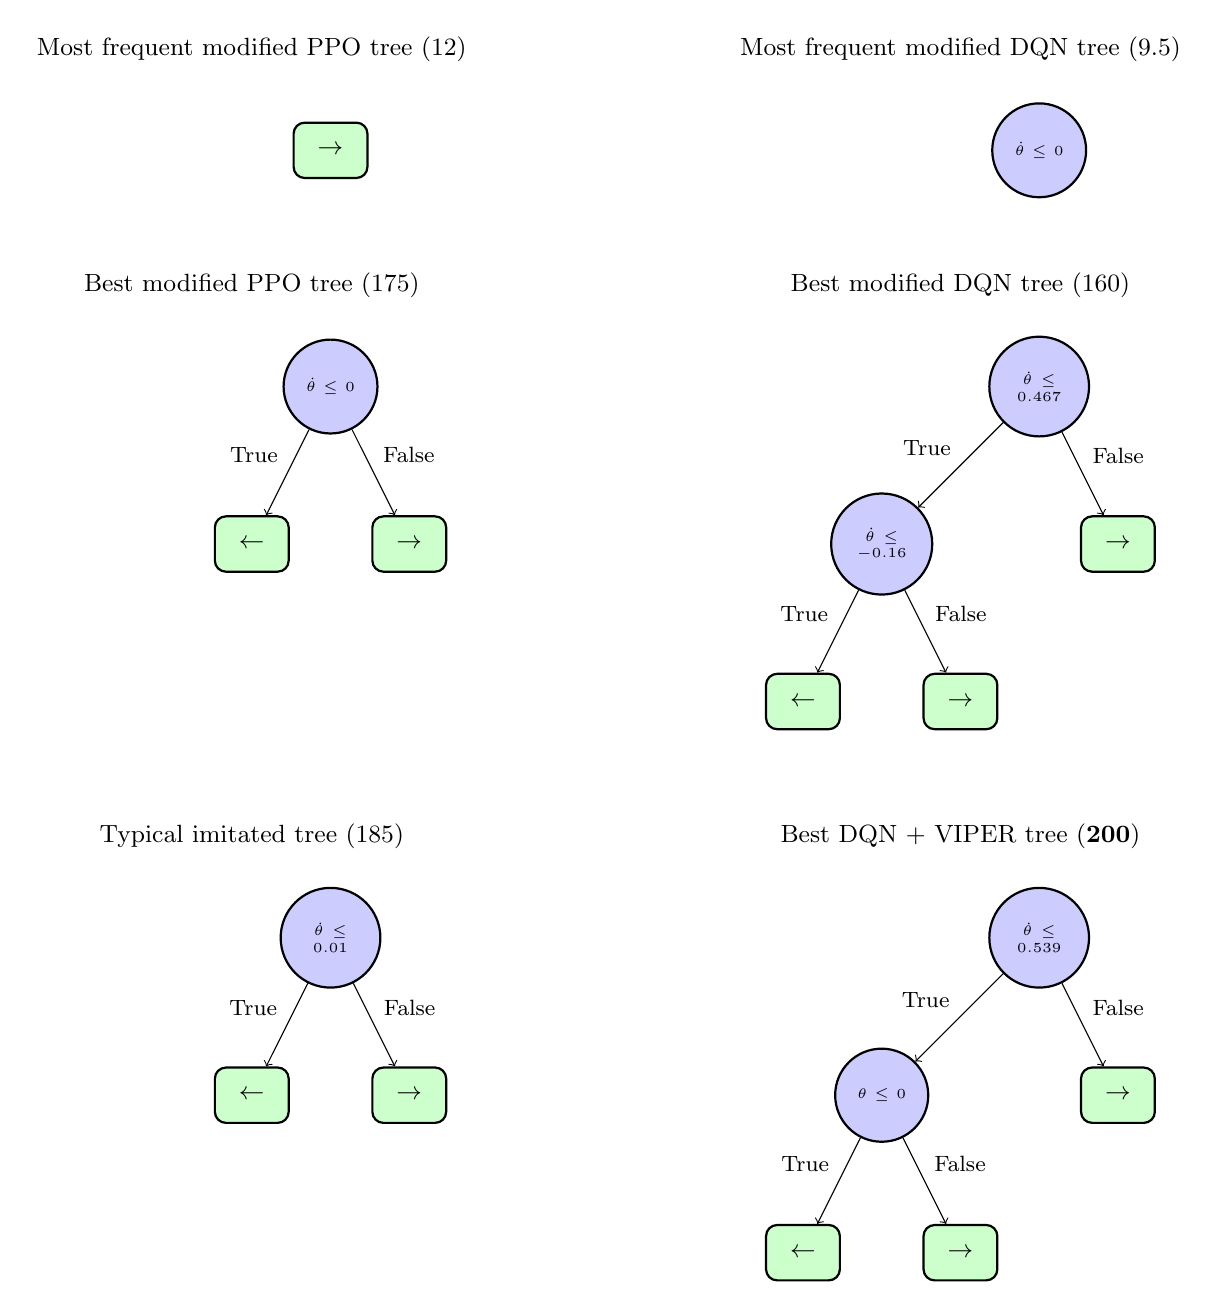
\begin{tikzpicture}[
        decision/.style={circle, draw, thick, fill=blue!20, text width=2.5em, text centered, minimum height=2.5em, font=\tiny},
        leaf/.style={rectangle, draw, thick, fill=green!20, text width=2em, text centered, rounded corners, minimum height=2em, font=\small},
        edge_label/.style={font=\footnotesize, midway}
    ]

        \node[leaf] (tree7_root) at (-3,3) {$\rightarrow$};
        % \draw[->] (tree7_root) to[out=45,in=0,looseness=5] (tree7_root);

        \node[decision] (tree7_root) at (6,3) {$\dot{\theta} \leq 0$};
        % \draw[->] (tree7_root) to[out=45,in=0,looseness=5] (tree7_root);
        
        % Tree 4: if x <= 0.5 move right else move left
        \node[decision] (tree4_root) at (-3,0) { $\dot{\theta}\leq 0$};
        \node[leaf] (tree4_right) at (-4,-2) {$\leftarrow$};
        \node[leaf] (tree4_left) at (-2,-2) {$\rightarrow$};
        \draw[->] (tree4_root) -- (tree4_right) node[edge_label, above left] {True};
        \draw[->] (tree4_root) -- (tree4_left) node[edge_label, above right] {False};
        

        % Tree 7: if x <= 0.5 and y <= 0.5 move right else move down
        \node[decision] (tree7_root) at (6,0) {$\dot{\theta}\leq 0.467$};
        \node[decision] (tree7_y) at (4,-2) {$\dot{\theta}\leq -0.16$};
        \node[leaf] (tree7_right) at (3,-4) {$\leftarrow$};
        \node[leaf] (tree7_down) at (5,-4) {$\rightarrow$};
        \node[leaf] (tree7_down2) at (7,-2) {$\rightarrow$};
        \draw[->] (tree7_root) -- (tree7_y) node[edge_label, above left] {True};
        \draw[->] (tree7_root) -- (tree7_down2) node[edge_label, above right] {False};
        \draw[->] (tree7_y) -- (tree7_right) node[edge_label, above left] {True};
        \draw[->] (tree7_y) -- (tree7_down) node[edge_label, above right] {False};




        % Tree 4: if x <= 0.5 move right else move left (Second row, left)
        \node[decision] (tree4_root2) at (-3,-7) { $\dot{\theta}\leq 0.01$};
        \node[leaf] (tree4_right2) at (-4,-9) {$\leftarrow$};
        \node[leaf] (tree4_left2) at (-2,-9) {$\rightarrow$};
        \draw[->] (tree4_root2) -- (tree4_right2) node[edge_label, above left] {True};
        \draw[->] (tree4_root2) -- (tree4_left2) node[edge_label, above right] {False};


        % Tree 7: if x <= 0.5 and y <= 0.5 move right else move down (Second row, right)
        \node[decision] (tree7_root2) at (6,-7) {$\dot{\theta}\leq 0.539$};
        \node[decision] (tree7_y2) at (4,-9) {$\theta\leq 0$};
        \node[leaf] (tree7_right2) at (3,-11) {$\leftarrow$};
        \node[leaf] (tree7_down3) at (5,-11) {$\rightarrow$};
        \node[leaf] (tree7_down4) at (7,-9) {$\rightarrow$};
        \draw[->] (tree7_root2) -- (tree7_y2) node[edge_label, above left] {True};
        \draw[->] (tree7_root2) -- (tree7_down4) node[edge_label, above right] {False};
        \draw[->] (tree7_y2) -- (tree7_right2) node[edge_label, above left] {True};
        \draw[->] (tree7_y2) -- (tree7_down3) node[edge_label, above right] {False};
        

        % Labels
        \node[above] at (-4,4) {{\small Most frequent modified PPO tree (12)}};
        \node[above] at (5,4) {{\small Most frequent modified DQN tree (9.5)}};

        \node[above] at (-4,1) {{\small Best modified PPO tree (175)}};
        \node[above] at (5,1) {{\small Best modified DQN tree (160)}};
        \node[above] at (-4,-6) {{\small Typical imitated tree (185)}};
        \node[above] at (5,-6) {{\small Best DQN + VIPER tree (\textbf{200})}};


    \end{tikzpicture}
    \caption{Trees obtained by modified deep RL in IBMDPs against trees obtained with imitation (RL objective value). $\theta$ and $\dot{\theta}$ are respectively the angle and the angular velocity of the pole}
    \label{fig:trees-drl}
\end{figure}


On figure~\ref{fig:ppo-trees}, we isolate the best performing algorithms instantiations that learn decision tree policies for the CartPole MDP.
We compare the best modified DQN and modified PPO to imitation learning baselines that use the surrogate imitation objective to find CartPole decision tree policies.
We find that despite having poor performances in \textit{average}, the modified deep reinforcement learning baselines can find very good decision tree policies as shown by the min-max shaded areas on the left of figure~\ref{fig:ppo-trees} and the corresponding estimated density of learned trees performances.
However this is not desirable, a user typically wants an algorithm that can consistently find good decision tree policies.
As shown by the estimated densities, indirect methods consistently find good decision tree policies (the higher modes of distributions are on the right of the plot).
On the other hand, the decision tree policies returned by direct RL methods seem equally distributed on both extremes of the scores.

On figure~\ref{fig:trees-drl}, we present the best decision tree policies for CartPole returned by modified DQN and modified PPO.
We used algorithm~\ref{alg:extract-tree} to extract 20 trees from the 20 memoryless policies returned by the modified deep reinforcement learning algorithms over the 20 training seeds.
We then plot the best tree for each baseline.
Those trees get an average RL objective of roughly 175.
Similarly, we plot a representative tree for imitation learning baseline as well as a tree that is optimal for CartPole w.r.t. the RL objective obtained with VIPER. 
Unlike for direct methods, the trees returned by imitation learning are extremely similar across seeds. In particular they often only vary in the scalar value used in the root node but in general have the same structure and test the angular velocity.
On the other hand the most frequent trees across seeds returned by modified RL baselines are ``trivial'' decision tree policies that either repeat the same downstream action forever or repeat the same IGA (definition~\ref{def:ibmdp}) forever.

\section{RL objective values calculations}\label{calcs}
\paragraph{Optimal depth-1 decision tree policy} $\pi_{\mathcal{T}_1}$ has one root node that tests $x\leq1$ (respectively $y\leq1$) and two leaf nodes $\rightarrow$ and $\downarrow$. 
    To compute $V^\pi_{\mathcal{T}_1}(\boldsymbol{o}_0)$, we compute the values of $\pi_{\mathcal{T}_1}$ in each of the possible starting states $(\boldsymbol{s}_0, \boldsymbol{o}_0), (\boldsymbol{s}_1, \boldsymbol{o}_0), (\boldsymbol{s}_2, \boldsymbol{o}_0), (\boldsymbol{s}_g, \boldsymbol{o}_0)$ and compute the expectation over those. 
    At initialization, when the downstream state is $\boldsymbol{s}_g = (1.5, 0.5)$, the depth-1 decision tree policy cycles between taking an information gathering action $x\leq1$ and moving down to get a positive reward for which it gets the returns:
    \begin{align*}
        V^{\pi_{\mathcal{T}_1}} (\boldsymbol{s}_g, \boldsymbol{o}_0) &= \zeta + \gamma + \gamma^2 \zeta + \gamma^3 \dots \\
        &= \overset{\infty}{\underset{t=0}\sum} \gamma^{2t} \zeta + \overset{\infty}{\underset{t=0}\sum} \gamma^{2t+1} \\
        &= \frac{\zeta + \gamma}{1 - \gamma^2}
    \end{align*}
    At initialization, in either of the downstream states $\boldsymbol{s}_0=(0.5,0.5)$ and $\boldsymbol{s}_2=(1.5, 1.5)$, the value of the depth-1 decision tree policy is the return when taking one information gathering action $x\leq1$, then moving right or down, then following the policy from the goal state $\boldsymbol{s}_g$:
    \begin{align*}
        V^{\pi_{\mathcal{T}_1}} (\boldsymbol{s}_0, o_0) &= \zeta + \gamma 0 + \gamma^2 V^{\pi_{\mathcal{T}_1}} (\boldsymbol{s}_g, o_0) \\
        &= \zeta + \gamma^2 V^{\pi_{\mathcal{T}_1}} (\boldsymbol{s}_g, o_0) \\
        &= V^{\pi_{\mathcal{T}_1}} (\boldsymbol{s}_2, o_0)
    \end{align*}
    Similarly, the value of the best depth-1 decision tree policy in state $\boldsymbol{s}_1=(0.5,1.5)$ is the value of taking one information gathering action then moving right to $\boldsymbol{s}_2$ then following the policy in $\boldsymbol{s}_2$:
    \begin{align*}
        V^{\pi_{\mathcal{T}_1}} (\boldsymbol{s}_1, \boldsymbol{o}_0) &= \zeta + \gamma 0 + \gamma^2 V^{\pi_{\mathcal{T}_1}} (\boldsymbol{s}_2, \boldsymbol{o}_0) \\
        &= \zeta + \gamma^2 V^{\pi_{\mathcal{T}_1}} (\boldsymbol{s}_2, o_0) \\
        &= \zeta + \gamma^2 (\zeta + \gamma^2 V^{\pi_{\mathcal{T}_1}} (\boldsymbol{s}_g, o_0)) \\
        &= \zeta + \gamma^2 \zeta + \gamma^4 V^{\pi_{\mathcal{T}_1}} (\boldsymbol{s}_g, o_0)
    \end{align*}
    Since the probability of being in any downstream states at initialization given that the observation is $\boldsymbol{o}_0$ is simply the probability of being in any downstream states at initialization, we can write:
    \begin{align*}
        V^{\pi_{\mathcal{T}_1}} (\boldsymbol{o}_0) &= \frac{1}{4} V^{\pi_{\mathcal{T}_1}} (\boldsymbol{s}_g, \boldsymbol{o}_0) + \frac{2}{4} V^{\pi_{\mathcal{T}_1}} (\boldsymbol{s}_2, \boldsymbol{o}_0) + \frac{1}{4} V^{\pi_{\mathcal{T}_1}} (\boldsymbol{s}_1, \boldsymbol{o}_0) \\
        &= \frac{1}{4} \frac{\zeta + \gamma}{1 - \gamma^2} + \frac{2}{4} (\zeta + \gamma^2 \frac{\zeta + \gamma}{1 - \gamma^2}) + \frac{1}{4} (\zeta + \gamma^2 \zeta + \gamma^4 \frac{\zeta + \gamma}{1 - \gamma^2}) \\
        &= \frac{1}{4} \frac{\zeta + \gamma}{1 - \gamma^2} + \frac{2}{4} (\frac{\zeta + \gamma ^ 3}{1-\gamma^2}) + \frac{1}{4}(\frac{\zeta+\gamma^5}{1-\gamma^2}) \\
        &= \frac{4\zeta + \gamma + 2\gamma^3 + \gamma^5}{4(1-\gamma^2)}
    \end{align*}

\paragraph{Depth-0 decision tree:} has only one leaf node that takes a single downstream action indefinitely.
For this type of tree the best reward achievable is to take actions that maximize the probability of reaching the objective $\rightarrow$ or $\downarrow$. In that case the objective value of such tree is:
In the goal state $G = (1, 0)$, the value of the depth-0 tree $\mathcal{T}_0$ is:
\begin{align*}
    V^{\mathcal{T}_0}_G &= 1 + \gamma + \gamma^2 + \dots \\
    &= \overset{\infty}{\underset{t=0}\sum} \gamma^t \\
    &= \frac{1}{1 - \gamma}
\end{align*}
In the state $(0, 0)$ when the policy repeats going right respectively in the state $(0, 1)$ when the policy repeats going down, the value is:
\begin{align*}
    V^{\mathcal{T}_0}_{S_0} &= 0 + \gamma V^{\mathcal{T}_0}_g \\
    &= \gamma V^{\mathcal{T}_0}_G
\end{align*}
In the other states the policy never gets positive rewards; $V^{\mathcal{T}_0}_{S_1} = V^{\mathcal{T}_0}_{S_2} = 0$. Hence:
\begin{align*}
J(\mathcal{T}_0) &= \frac{1}{4} V^{\mathcal{T}_0}_G + \frac{1}{4} V^{\mathcal{T}_0}_{S_0}+ \frac{1}{4} V^{\mathcal{T}_0}_{S_1}+ \frac{1}{4} V^{\mathcal{T}_0}_{S_2} \\
&= \frac{1}{4} V^{\mathcal{T}_0}_G + \frac{1}{4} \gamma V^{\mathcal{T}_0}_G + 0 + 0\\
&= \frac{1}{4} \frac{1}{1 - \gamma} + \frac{1}{4} \gamma \frac{1}{1 - \gamma} \\
&= \frac{1 + \gamma}{4(1 - \gamma)}
\end{align*}

\paragraph{Unbalanced depth-2 decision tree:}the unbalanced depth-2 decision tree  takes an information gathering action $x\leq0.5$ then either takes the $\downarrow$ action or takes a second information $y\leq0.5$ followed by $\rightarrow$ or $\downarrow$.
In states $G$ and $S_2$, the value of the unbalanced tree is the same as for the depth-1 tree.
In states $S_0$ and $S_1$, the policy takes two information gathering actions before taking a downstream action and so on:
\begin{align*}
    V^{\mathcal{T}_{u}}_{S_0} &= \zeta + \gamma \zeta + \gamma ^ 2 0 + \gamma ^ 3 V^{\mathcal{T}_1}_G
\end{align*} 
\begin{align*}
    V^{\mathcal{T}_{u}}_{S_1} &= \zeta + \gamma \zeta + \gamma ^ 2 0 + \gamma ^ 3 V^{\mathcal{T}_u}_{S_0} \\ 
    &= \zeta + \gamma \zeta + \gamma ^ 2 0 + \gamma ^ 3 (\zeta + \gamma \zeta + \gamma ^ 2 0 + \gamma ^ 3 V^{\mathcal{T}_1}_G) \\
    &= \zeta + \gamma \zeta + \gamma ^ 3 \zeta + \gamma ^ 4 \zeta + \gamma ^ 6 V^{\mathcal{T}_1}_G
\end{align*}
We get:
\begin{align*}
    J(\mathcal{T}_{u}) &= \frac{1}{4} V^{\mathcal{T}_u}_G + \frac{1}{4} V^{\mathcal{T}_u}_{S_0} + \frac{1}{4}V^{\mathcal{T}_u}_{S_1} + \frac{1}{4}V^{\mathcal{T}_u}_{S_2} \\
    &=  \frac{1}{4} V^{\mathcal{T}_1}_G + \frac{1}{4}(\zeta + \gamma \zeta + \gamma ^ 3 V^{\mathcal{T}_1}_G) + \frac{1}{4} (\zeta + \gamma \zeta + \gamma ^ 3 \zeta + \gamma ^ 4 \zeta + \gamma ^ 6 V^{\mathcal{T}_1}_G) + \frac{1}{4}V^{\mathcal{T}_1}_{S_2} \\
    &= \frac{1}{4} (\frac{\zeta + \gamma}{1-\gamma^2}) + \frac{1}{4}(\frac{\gamma\zeta + \gamma^4 + \zeta -\gamma^2\zeta}{1-\gamma^2}) + \frac{1}{4} (\zeta + \gamma \zeta + \gamma ^ 3 \zeta + \gamma ^ 4 \zeta + \gamma ^ 6 V^{\mathcal{T}_1}_G) + \frac{1}{4}V^{\mathcal{T}_1}_{S_2} \\
    &= \frac{1}{4} (\frac{\zeta + \gamma}{1-\gamma^2}) + \frac{1}{4}(\frac{\gamma\zeta + \gamma^4 + \zeta -\gamma^2\zeta}{1-\gamma^2}) + \frac{1}{4} (\frac{\zeta + \gamma\zeta -\gamma^2\zeta-\gamma^5\zeta+\gamma^6\zeta+\gamma^7}{1-\gamma^2}) + \frac{1}{4}V^{\mathcal{T}_1}_{S_2} \\
    &= \frac{1}{4} (\frac{\zeta + \gamma}{1-\gamma^2}) + \frac{1}{4}(\frac{\gamma\zeta + \gamma^4 + \zeta -\gamma^2\zeta}{1-\gamma^2}) + \frac{1}{4} (\frac{\zeta + \gamma\zeta -\gamma^2\zeta-\gamma^5\zeta+\gamma^6\zeta+\gamma^7}{1-\gamma^2}) + \frac{1}{4}(\frac{\zeta + \gamma ^ 3}{1-\gamma^2}) \\
    &= \frac{\zeta(4+2\gamma-2\gamma^2-\gamma^5+\gamma^6)+\gamma+\gamma^3+\gamma^4+\gamma^7}{4(1-\gamma^2)}
\end{align*}
\paragraph{The balanced depth-2 decision tree:}alternates in every state between taking the two available information gathering actions and then a downstream action.
The value of the policy in the goal state is:
\begin{align*}
    V^{\mathcal{T}_2}_{G} &= \zeta + \gamma\zeta + \gamma^2 + \gamma^3\zeta + \gamma^4\zeta + \dots \\
    &= \overset{\infty}{\underset{t=0}\sum} \gamma^{3t}\zeta + \overset{\infty}{\underset{t=0}\sum} \gamma^{3t+1}\zeta + \overset{\infty}{\underset{t=0}\sum} \gamma^{3t+2} \\
    &= \frac{\zeta}{1-\gamma^3} + \frac{\gamma\zeta}{1-\gamma^3} + \frac{\gamma^2}{1-\gamma^3}
\end{align*}
Following the same reasoning for other states we find the objective value for the depth-2 decision tree policy to be:
\begin{align*}
    J(\mathcal{T}_2) &=\frac{1}{4} V^{\mathcal{T}_2}_G + \frac{2}{4} V^{\mathcal{T}_2}_{S_2} + \frac{1}{4} V^{\mathcal{T}_2}_{S_1} \\
    &= \frac{1}{4} V^{\mathcal{T}_2}_G + \frac{2}{4}(\zeta + \gamma\zeta + \gamma^2 0 + \gamma^3V^{\mathcal{T}_2}_G) + \frac{1}{4} (\zeta+\gamma\zeta+\gamma^2 0 + \gamma^3\zeta+\gamma^4\zeta+\gamma^5 0 +\gamma^6 V^{\mathcal{T}_2}_G) \\
    &= \frac{\zeta(3+3\gamma)+\gamma^2+\gamma^5+\gamma^8}{4(1-\gamma^3)}
\end{align*}
\paragraph{Infinite tree:} we also consider the infinite tree policy that repeats an information gathering action forever and has objective: $J(\mathcal{T_{\text{inf}}}) = \frac{\zeta}{1-\gamma}$

\paragraph{Stochastic policy:} the other non-trivial policy that can be learned by solving a partially observable IBMDP is the stochastic policy that guarantees to reach $G$ after some time: fifty percent chance to do $\rightarrow$ and fifty percent chance to do $\downarrow$.
This stochastic policy has objective value:
\begin{align*}
    V^{\text{stoch}}_G &= \frac{1}{1-\gamma} \\
    V^{\text{stoch}}_{S_0} &= 0 + \frac{1}{2}\gamma V^{\text{stoch}}_G + \frac{1}{2}\gamma V^{\text{stoch}}_{S_1} \\
    V^{\text{stoch}}_{S_2} &= 0 + \frac{1}{2}\gamma V^{\text{stoch}}_G + \frac{1}{2}\gamma V^{\text{stoch}}_{S_1} = V^{\text{stoch}}_{S_0} \\
    V^{\text{stoch}}_{S_1} &= 0 + \frac{1}{2}\gamma V^{\text{stoch}}_{S_2} + \frac{1}{2}\gamma V^{\text{stoch}}_G = \frac{1}{2}\gamma V^{\text{stoch}}_{S_0} + \frac{1}{2}\gamma V^{\text{stoch}}_G
\end{align*}
Solving these equations:
\begin{align*}
    V^{\text{stoch}}_{S_1} &= \frac{1}{2}\gamma V^{\text{stoch}}_{S_0} + \frac{1}{2}\gamma V^{\text{stoch}}_G \\
    &= \frac{1}{2}\gamma (\frac{1}{2}\gamma V^{\text{stoch}}_G + \frac{1}{2}\gamma V^{\text{stoch}}_{S_1}) + \frac{1}{2}\gamma V^{\text{stoch}}_G \\
    &= \frac{1}{4}\gamma^2 V^{\text{stoch}}_G + \frac{1}{4}\gamma^2 V^{\text{stoch}}_{S_1} + \frac{1}{2}\gamma V^{\text{stoch}}_G \\
    V^{\text{stoch}}_{S_1} - \frac{1}{4}\gamma^2 V^{\text{stoch}}_{S_1} &= \frac{1}{4}\gamma^2 V^{\text{stoch}}_G + \frac{1}{2}\gamma V^{\text{stoch}}_G \\
    V^{\text{stoch}}_{S_1}(1 - \frac{1}{4}\gamma^2) &= (\frac{1}{4}\gamma^2 + \frac{1}{2}\gamma) V^{\text{stoch}}_G \\
    V^{\text{stoch}}_{S_1} &= \frac{\frac{1}{4}\gamma^2 + \frac{1}{2}\gamma}{1 - \frac{1}{4}\gamma^2} V^{\text{stoch}}_G \\
    &= \frac{\gamma(\frac{1}{4}\gamma + \frac{1}{2})}{1 - \frac{1}{4}\gamma^2} \cdot \frac{1}{1-\gamma} \\
    &= \frac{\gamma(\frac{1}{4}\gamma + \frac{1}{2})}{(1 - \frac{1}{4}\gamma^2)(1-\gamma)}
\end{align*}
\begin{align*}
    V^{\text{stoch}}_{S_0} &= \frac{1}{2}\gamma V^{\text{stoch}}_G + \frac{1}{2}\gamma V^{\text{stoch}}_{S_1} \\
    &= \frac{1}{2}\gamma \cdot \frac{1}{1-\gamma} + \frac{1}{2}\gamma \cdot \frac{\gamma(\frac{1}{4}\gamma + \frac{1}{2})}{(1 - \frac{1}{4}\gamma^2)(1-\gamma)} \\
    &= \frac{\frac{1}{2}\gamma}{1-\gamma} + \frac{\frac{1}{2}\gamma^2(\frac{1}{4}\gamma + \frac{1}{2})}{(1 - \frac{1}{4}\gamma^2)(1-\gamma)} \\
    &= \frac{\frac{1}{2}\gamma(1 - \frac{1}{4}\gamma^2) + \frac{1}{2}\gamma^2(\frac{1}{4}\gamma + \frac{1}{2})}{(1 - \frac{1}{4}\gamma^2)(1-\gamma)} \\
    &= \frac{\frac{1}{2}\gamma - \frac{1}{8}\gamma^3 + \frac{1}{8}\gamma^3 + \frac{1}{4}\gamma^2}{(1 - \frac{1}{4}\gamma^2)(1-\gamma)} \\
    &= \frac{\frac{1}{2}\gamma + \frac{1}{4}\gamma^2}{(1 - \frac{1}{4}\gamma^2)(1-\gamma)} \\
    &= \frac{\gamma(\frac{1}{2} + \frac{1}{4}\gamma)}{(1 - \frac{1}{4}\gamma^2)(1-\gamma)}
\end{align*}
\begin{align*}
    J(\mathcal{T}_{\text{stoch}}) &= \frac{1}{4}(V^{\text{stoch}}_G + V^{\text{stoch}}_{S_0} + V^{\text{stoch}}_{S_1} + V^{\text{stoch}}_{S_2}) \\
    &= \frac{1}{4}\left(\frac{1}{1-\gamma} + 2 \cdot \frac{\gamma(\frac{1}{2} + \frac{1}{4}\gamma)}{(1 - \frac{1}{4}\gamma^2)(1-\gamma)} + \frac{\gamma(\frac{1}{4}\gamma + \frac{1}{2})}{(1 - \frac{1}{4}\gamma^2)(1-\gamma)}\right) \\
    &= \frac{1}{4}\left(\frac{1}{1-\gamma} + \frac{2\gamma(\frac{1}{2} + \frac{1}{4}\gamma) + \gamma(\frac{1}{4}\gamma + \frac{1}{2})}{(1 - \frac{1}{4}\gamma^2)(1-\gamma)}\right) \\
    &= \frac{1}{4}\left(\frac{1}{1-\gamma} + \frac{\gamma + \frac{1}{2}\gamma^2 + \frac{1}{4}\gamma^2 + \frac{1}{2}\gamma}{(1 - \frac{1}{4}\gamma^2)(1-\gamma)}\right) \\
    &= \frac{1}{4}\left(\frac{1}{1-\gamma} + \frac{\frac{3}{2}\gamma + \frac{3}{4}\gamma^2}{(1 - \frac{1}{4}\gamma^2)(1-\gamma)}\right) \\
    &= \frac{1}{4}\left(\frac{1 - \frac{1}{4}\gamma^2 + \frac{3}{2}\gamma + \frac{3}{4}\gamma^2}{(1 - \frac{1}{4}\gamma^2)(1-\gamma)}\right) \\
    &= \frac{1}{4}\left(\frac{1 + \frac{3}{2}\gamma + \frac{1}{2}\gamma^2}{(1 - \frac{1}{4}\gamma^2)(1-\gamma)}\right) \\
    &= \frac{1 + \frac{3}{2}\gamma + \frac{1}{2}\gamma^2}{4(1 - \frac{1}{4}\gamma^2)(1-\gamma)}
\end{align*}

\section{Training curves}\label{sec:training}
We plot the sub-optimality gaps during training, w.r.t. the RL objective (definition~\ref{def:mdp-obj}), between the learned memoryless policy and the optimal deterministic memoryless policy: $|\mathbb{E}\left[V^\pi^{\star}(\boldsymbol{s}_0,\boldsymbol{o}_0)| \boldsymbol{s}_0\sim T_0\right] - \mathbb{E}\left[V^\pi(\boldsymbol{s}_0,\boldsymbol{o}_0)|\boldsymbol{s}_0\sim T_0\right]|$.
Because we know the whole POIBMDP model that we can represent exactly as tables, and because we know for each $\zeta$ the RL objective value of the optimal deterministic memoryless policy (figure~\ref{fig:irl-objectives}), we can report the \textit{exact} sub-optimality gaps.
In figure~\ref{fig:rl-poibmdp}, we plot the sub-optimality gaps--averaged over 100 seeds--of learned policies during training.
We do so for 200 different POIBMDPs where we change the reward for information gathering actions: we sample 200 $\zeta$ values uniformly in $[-1, 2]$.
In figure~\ref{fig:rl-poibmdp}, a different color represents a different POIBMDP.

Recall from figure~\ref{fig:irl-objectives} that for: (i) $\zeta\in [-1, 0]$, the optimal deterministic memoryless policy is a depth-0 tree, (ii) $\zeta\in ]0, 1[$, the optimal deterministic memoryless policy is a depth-1 tree, and (iii) $\zeta\in [1, 2]$, the optimal deterministic memoryless policy is a ``infinite'' tree that contains infinite number of internal nodes.
We observe that, despite all sub-optimality gaps converging independently of the $\zeta$ values, not all algorithms in all POIBMDPs fully minimize the sub-optimality gap.
In particular, all algorithms seem to consistently minimize the gap, i.e. learn the optimal policy or Q-function, only for $\zeta \in [1, 2]$ (all the yellow lines go to 0).
However, we are interested in the range $\zeta\in ]0, 1[$ where the optimal decision tree policy is non-trivial, i.e. not taking the same action forever.
In that range, no baseline consistently minimizes the sub-optimality gap.
\begin{figure}
    \centering
    \includegraphics[width=0.7\textwidth]{../images/images_part1/learning_curves.pdf}
    \caption{(Asymmetric) reinforcement learning in POIBMDPs. 
    In each subplot, each single line is colored by the value of $\zeta$ in the corresponding POIBMDP in which learning occurs. 
    Each single learning curve represent the sub-optimality gap averaged over 100 seeds.
    }\label{fig:rl-poibmdp}
\end{figure}

\begin{figure}
    \centering
    \includegraphics[width=1\textwidth]{../images/images_part1/tree_distributions.pdf}
    \caption{Distributions of final tree policies learned across the 100 seeds.
    For each $\zeta$ value, there are four colored points. Each point represent the share of depth-0 trees (red), depth-1 trees (green), unbalanced depth-2 trees (orange) and depth-2 trees (blue).
    }\label{fig:dt-distrib-poibmdp}
\end{figure}

\section{Tabular RL algorithmic details for POIBMDPs}\label{sec:hp-pomdp}

\RestyleAlgo{ruled}
\SetKwComment{Comment}{}{}
\begin{algorithm}
    \KwData{A POMDP, learning rates $\alpha_u,\ \alpha_q$, exploration prob. $\epsilon$}
    \KwResult{$\pi:O\rightarrow A$}
    \textcolor{teal}{Initialize $U(\boldsymbol{x},a) = 0$ for all $x \in X, a \in A$ \\}
    Initialize $Q(\boldsymbol{o},a) = 0$ for all $o \in O, a \in A$ \\
    \For{each episode}{
        Initialize state $x_0 \sim T_0$ \\
        Initialize observation $\boldsymbol{o}_0 \sim \Omega(\boldsymbol{x}_0)$ \\

        \For{each step $t$}{
            Choose action $a_t$ using $\epsilon$-greedy: $a_t = \operatorname{argmax}_a Q(\boldsymbol{o}_t,a)$ with prob. $1-\epsilon$ \\
            Take action $a_t$, observe $r_t = R(\boldsymbol{x}_t,a_t)$, $x_{t+1} \sim T(x_t,a_t)$, and $\boldsymbol{o}_{t+1} \sim \Omega(\boldsymbol{x}_{t+1})$ \\
            \textcolor{teal}{$y \leftarrow r + \gamma U(\boldsymbol{x}_{t+1}, \operatorname{argmax}_{a'} Q(\boldsymbol{o}_{t+1}, a'))$} \\
            $U(\boldsymbol{x}_t,a_t) \leftarrow (1 - \alpha_u) U(\boldsymbol{x}_t, a_t) + \alpha_u y $ \\
            \textcolor{teal}{$Q(\boldsymbol{o}_t,a_t) \leftarrow (1 - \alpha_q) Q(\boldsymbol{o}_t, a_t) + \alpha_q y $} \\
            $x_t \leftarrow \boldsymbol{x}_{t+1}$ \\
            $\boldsymbol{o}_t \leftarrow \boldsymbol{o}_{t+1}$ \\
        }
    }
    $\pi(o) = \operatorname{argmax}_a Q(\boldsymbol{o},a)$
    \caption{Asymmetric Q-Learning. We highlight in green the differences with the standard Q-learning~\cite{watkins1992q}}\label{alg:asymqlearning}
\end{algorithm}

\RestyleAlgo{ruled}
\SetKwComment{Comment}{}{}
\begin{algorithm}
    \KwData{POMDP $\mathcal{M}_{po} = \langle X, O, A, R, T, T_0, \Omega \rangle$, learning rates $\alpha_u,\quad \alpha_q$, exploration rate $\epsilon$}
    \KwResult{$\pi:O\rightarrow A$}
    Initialize $U(x,a) = 0$ for all $x \in X, a \in A$ \\
    Initialize $Q(o,a) = 0$ for all $o \in O, a \in A$ \\

    \For{each episode}{
        Initialize state $x_0 \sim T_0$ \\
        Initialize observation $\boldsymbol{o}_0 \sim \Omega(x_0)$ \\
        Choose action $a_0$ using $\epsilon$-greedy: $a_0 = \operatorname{argmax}_a Q(\boldsymbol{o}_0,a)$ with prob. $1-\epsilon$ \\

        \For{each step $t$}{
            Take action $a_t$, observe $r_t = R(x_t,a_t)$, $x_{t+1} \sim T(x_t,a_t)$, and $\boldsymbol{o}_{t+1} \sim \Omega(x_{t+1})$ \\
            Choose action $a_{t+1}$ using $\epsilon$-greedy: $a_{t+1} = \operatorname{argmax}_a Q(\boldsymbol{o}_{t+1},a)$ with prob. $1-\epsilon$ \\
            $y \leftarrow r + \gamma U(x_{t+1}, a_{t+1})$ \Comment{// TD target using actual next action} \\
            $U(x_t,a_t) \leftarrow (1 - \alpha_u) U(x_t, a_t) + \alpha_u y $ \\
            $Q(\boldsymbol{o}_t,a_t) \leftarrow (1 - \alpha_q) Q(\boldsymbol{o}_t, a_t) + \alpha_q y $ \\
            $x_t \leftarrow x_{t+1}$ \\
            $\boldsymbol{o}_t \leftarrow \boldsymbol{o}_{t+1}$ \\
            $a_t \leftarrow a_{t+1}$ \\
        }
    }
    $\pi(b\oldsymbol{o}) = \operatorname{argmax}_a Q(\boldsymbol{o},a)$ \Comment{// Extract greedy policy}
    \caption{Asymmetric Sarsa}\label{alg:asymsarsa}
\end{algorithm}

\RestyleAlgo{ruled}
\SetKwComment{Comment}{}{}
\begin{algorithm}
    \KwData{POMDP $\mathcal{M}_{po} = \langle X, O, A, R, T, T_0, \Omega \rangle$, learning rate $\alpha$, policy parameters $\theta$, number of trajectories $N$}
    \KwResult{Stochastic partially observable policy $\pi_\theta: O\rightarrow \Delta(A)$}
    Initialize policy parameters $\theta$ \\
    Initialize $Q(\boldsymbol{o}, a) = 0$ for all observations $o$ and actions $a$ \\
    \For{each episode}{
        \For{$i = 1$ to $N$}{
            Generate trajectory $\tau_i = (\boldsymbol{s}_0, a_0, r_0, \boldsymbol{s}_1, a_1, r_1, \ldots, \boldsymbol{s}_T)$ following $\pi_\theta$ \\
            \For{each timestep $t$ in trajectory $\tau_i$}{
                $G_t \leftarrow \sum_{k=t}^{T} \gamma^{k-t} r_k$ \Comment{// Compute return}
                Store $(\boldsymbol{o}_t, a_t, G_t)$ for later averaging
            }
        }
        \For{each unique observation-action pair $(o, a)$}{
            $Q(o, a) \leftarrow \frac{1}{|\{(\boldsymbol{o}, a)\}|} \sum_{(\boldsymbol{o}, a, G)} G$ \Comment{// Monte Carlo estimate}
        }
        \For{each observation $o$}{
            \For{each action $a$}{
                $\pi_1(a|\boldsymbol{o}) \leftarrow 1.0$ if $a = \operatorname{argmax}_{a'} Q(\boldsymbol{o}, a')$, $0.0$ otherwise \Comment{// Deterministic policy from Q-values}
                $\pi(a|\boldsymbol{o}) \leftarrow (1 - \alpha) \pi(a|\boldsymbol{o}) + \alpha \pi_1(a|\boldsymbol{o}o)$ \Comment{// Policy improvement step}
            }
        }
        Reset $Q(\boldsymbol{o}, a) = 0$ for all observations $\boldsymbol{o}$ and actions $a$ \Comment{// Reset for next episode}
    }
    \caption{Asymmetric policy gradient algorithm. Uses Monte Carlo estimates of the average reward value functions to perform policy improvements.}\label{alg:jsj}
\end{algorithm}

\begin{table}
    \centering
    \caption{Summary of RL baselines Hyperparameters}\label{tab:ib-params}
    \small
    \begin{tabular}{llr}
    \toprule
    \textbf{algorithm} & \textbf{Problem} & \textbf{Hyperparameters comb.} \\
    \midrule
    Policy Gradient & PO/IB/MDP & 420 \\
    JSJ & POIBMDP & 15 \\
    Q-learning & PO/IB/MDP & 192 \\
    Asym Q-learning & POIBMDP & 768 \\
    Sarsa & PO/IB/MDP & 192 \\
    Asym Sarsa & POIBMDP & 768 \\
    \bottomrule
    \end{tabular}
    \end{table}

\begin{table}
\small
\centering
\caption{PG Hyperparameter Space (140 combinations)}
\begin{tabular}{lll}
\toprule
\textbf{Hyperparameter} & \textbf{Values} & \textbf{Description} \\
\midrule
Learning Rate (lr) & 0.001, 0.005, 0.01, 0.05, 0.1 & Policy gradient step size \\
Entropy Regularization (tau) & -1.0, -0.1, -0.01, 0.0, 0.01, 0.1, 1.0 & Entropy regularization coefficient \\
Temperature (eps) & 0.01, 0.1, 1.0, 10 & Softmax temperature \\
Episodes per Update (n\_steps) & 20, 200, 2000 & Number of episodes per policy update \\
\bottomrule
\end{tabular}
\end{table}

\begin{table}
\small
\centering
\caption{PG-IBMDP Hyperparameter Space (140 combinations)}
\begin{tabular}{lll}
\toprule
\textbf{Hyperparameter} & \textbf{Values} & \textbf{Description} \\
\midrule
Learning Rate (lr) & 0.001, 0.005, 0.01, 0.05, 0.1 & Policy gradient step size \\
Entropy Regularization (tau) & -1.0, -0.1, -0.01, 0.0, 0.01, 0.1, 1.0 & Entropy regularization coefficient \\
Temperature (eps) & 0.01, 0.1, 1.0, 10 & Softmax temperature \\
Episodes per Update (n\_steps) & 10, 100, 1000 & Number of episodes per policy update \\
\bottomrule
\end{tabular}
\end{table}


\begin{table}
\small
\centering
\caption{QL Hyperparameter Space (192 combinations)}
\begin{tabular}{lll}
\toprule
\textbf{Hyperparameter} & \textbf{Values} & \textbf{Description} \\
\midrule
Epsilon Schedules & (0.3, 1), (0.3, 0.99), (1, 1) & Initial exploration and decrease rate \\
Epsilon Schedules & (0.1, 1), (0.1, 0.99), (0.3, 0.99) & Initial exploration and decrease rate \\
Lambda & 0.0, 0.3, 0.6, 0.9 & Eligibility trace decay \\
Learning Rate (lr\_o) & 0.001, 0.005, 0.01, 0.1 & Observation Q-learning rate \\
Optimistic & True, False & Optimistic initialization \\
\bottomrule
\end{tabular}
\end{table}

\begin{table}
\small
\centering
\caption{QL-Asym Hyperparameter Space (768 combinations)}
\begin{tabular}{lll}
\toprule
\textbf{Hyperparameter} & \textbf{Values} & \textbf{Description} \\
\midrule
Epsilon Schedules & (0.3, 1), (0.3, 0.99), (1, 1) & Initial exploration and decrease rate \\
Epsilon Schedules & (0.1, 1), (0.1, 0.99), (0.3, 0.99) & Initial exploration and decrease rate \\
Lambda & 0.0, 0.3, 0.6, 0.9 & Eligibility trace decay \\
Learning Rate (lr\_o) & 0.001, 0.005, 0.01, 0.1 & Observation Q-learning rate \\
Learning Rate (lr\_v) & 0.001, 0.005, 0.01, 0.1 & State-action Q-learning rate \\
Optimistic & True, False & Optimistic initialization \\
\bottomrule
\end{tabular}
\end{table}

\begin{table}
\small
\centering
\caption{QL-IBMDP Hyperparameter Space (192 combinations)}
\begin{tabular}{lll}
\toprule
\textbf{Hyperparameter} & \textbf{Values} & \textbf{Description} \\
\midrule
Epsilon Schedules & (0.3, 1), (0.3, 0.99), (1, 1) & Initial exploration and decrease rate \\
Epsilon Schedules & (0.1, 1), (0.1, 0.99), (0.3, 0.99) & Initial exploration and decrease rate \\
Lambda & 0.0, 0.3, 0.6, 0.9 & Eligibility trace decay \\
Learning Rate (lr\_v) & 0.001, 0.005, 0.01, 00.1 & State-action Q-learning rate \\
Optimistic & True, False & Optimistic initialization \\
\bottomrule
\end{tabular}
\end{table}

\begin{table}
\small
\centering
\caption{SARSA Hyperparameter Space (192 combinations)}
\begin{tabular}{lll}
\toprule
\textbf{Hyperparameter} & \textbf{Values} & \textbf{Description} \\
\midrule
Epsilon Schedules & (0.3, 1), (0.3, 0.99), (1, 1) & Initial exploration and decrease rate \\
Epsilon Schedules & (0.1, 1), (0.1, 0.99), (0.3, 0.99) & Initial exploration and decrease rate \\
Lambda & 0.0, 0.3, 0.6, 0.9 & Eligibility trace decay \\
Learning Rate (lr\_o) & 0.001, 0.005, 0.01, 0.1 & Observation SARSA learning rate \\
Optimistic & True, False & Optimistic initialization \\
\bottomrule
\end{tabular}
\end{table}

\begin{table}
\small
\centering
\caption{SARSA-Asym Hyperparameter Space (768 combinations)}
\begin{tabular}{lll}
\toprule
\textbf{Hyperparameter} & \textbf{Values} & \textbf{Description} \\
\midrule
Epsilon Schedules & (0.3, 1), (0.3, 0.99), (1, 1) & Initial exploration and decrease rate \\
Epsilon Schedules & (0.1, 1), (0.1, 0.99), (0.3, 0.99) & Initial exploration and decrease rate \\
Lambda & 0.0, 0.3, 0.6, 0.9 & Eligibility trace decay \\
Learning Rate (lr\_o) & 0.001, 0.005, 0.01, 0.1 & Observation SARSA learning rate \\
Learning Rate (lr\_v) & 0.001, 0.005, 0.01, 0.1 & State-action SARSA learning rate \\
Optimistic & True, False & Optimistic initialization \\
\bottomrule
\end{tabular}
\end{table}

\begin{table}
\small
\centering
\caption{SARSA-IBMDP Hyperparameter Space (192 combinations)}
\begin{tabular}{lll}
\toprule
\textbf{Hyperparameter} & \textbf{Values} & \textbf{Description} \\
\midrule
Epsilon Schedules & (0.3, 1), (0.3, 0.99), (1, 1) & Initial exploration and decrease rate \\
Epsilon Schedules & (0.1, 1), (0.1, 0.99), (0.3, 0.99) & Initial exploration and decrease rate \\
Lambda & 0.0, 0.3, 0.6, 0.9 & Eligibility trace decay \\
Learning Rate (lr\_v) & 0.001, 0.005, 0.01, 0.1 & State-action SARSA learning rate \\
Optimistic & True, False & Optimistic initialization \\
\bottomrule
\end{tabular}
\end{table}

\begin{table}
\centering
\small
\caption{Asymmetric sarsa hyperparameters (768 combinations each run 10 times)}\label{tab:hp-sarsa}
\begin{tabular}{lll}
\toprule
\textbf{Hyperparameter} & \textbf{Values} & \textbf{Description} \\
\midrule
Epsilon Schedules & (0.3, 1), (0.3, 0.99), (1, 1) & Initial exploration and decrease rate \\
Epsilon Schedules & (0.1, 1), (0.1, 0.99), (0.3, 0.99) & Initial exploration and decrease rate \\
Lambda & 0.0, 0.3, 0.6, 0.9 & Eligibility trace decay \\
Learning Rate $U$ & 0.001, 0.005, 0.01, 0.1 & learning rate for \\
 & & the Q-function \\
Learning Rate $Q$ & 0.001, 0.005, 0.01, 0.1 & learning rate for the \\
 & & partial observation dependent Q-function \\
Optimistic & True, False & Optimistic initialization \\
\bottomrule
\end{tabular}
\end{table}

\subsection{Training with the best hyperparameters}
\begin{table}
    \centering
    \begin{tabular}{|l|c|c|c|}
    \textbf{Hyperparameter} & \textbf{Asym Q-learning (10/10)} & \textbf{Asym Sarsa (10/10)} & \textbf{PG (4/10)} \\
    \toprule
    epsilon\_start & 1.0 & 1.0 & - \\
    epsilon\_decay & 0.99 & 0.99 & - \\
    batch\_size & 1 & 1 & - \\
    lambda\_ & 0.0 & 0.0 & - \\
    lr\_o & 0.01 & 0.1 & - \\
    lr\_v & 0.1 & 0.005 & - \\
    optimistic & False & False & - \\
    lr & - & - & 0.05 \\
    tau & - & - & 0.1 \\
    eps & - & - & 0.1 \\
    n\_steps & - & - & 2000 \\
    \bottomrule
    \end{tabular}
    \caption{Best hyperparameters for each algorithm on the POIBMDP problem}
    \label{tab:algorithm-hyperparameters}
    \end{table}

\begin{figure}
    \begin{subfigure}[b]{0.49\textwidth}
        \includegraphics[width=\textwidth]{../images/images_part1/ql_asym_best_learning_curves.pdf}
        \caption{Learning curves for asymmetric Q-learning with good hyperparameters.}
        \label{fig:best-learning-curves}
    \end{subfigure}
    \hfill
    \begin{subfigure}[b]{0.45\textwidth}
        \includegraphics[width=\textwidth]{../images/images_part1/ql_asym_best_tree_distributions.pdf}
        \caption{Trees distributions for asymmetric Q-learning with good hyperparameters}
        \label{fig:best-tree-distributions}
    \end{subfigure}
    \caption{Analysis of the top-performing asymmetric Q-learning instantiation. (left) Learning curves, and (right) tree distributions across different POIBMDP configurations.}
    \label{fig:asym-ql-analysis}
\end{figure}

\section{POIBMDPs for classification tasks}\label{sec:classif}
Let us show that, POIBMDPs associated with MDPs encoding supervised learning tasks, are in fact MDPs themselves.
Let us define such supervised learning MDPs in the context of a classification task (this definition extends trivially to regression tasks).
\begin{definition}[Classification Markov decision process]\label{def:cmdp}
    Given a set of $N$ examples denoted $\mathcal{E} = {\{(\boldsymbol{x}_i, y_i)\}}_{i=1}^N$ where each datum $\boldsymbol{x}_i \in \mathcal{X}$ is described by a set of $p$ features $x_{ij}$ with $1\leq j \leq p$, and $y_i \in \mathbb{Z}^m$ is the label associated with $\boldsymbol{x}_i$, a classification Markov decision Process is an MDP $\langle S, A, R, T, T_0 \rangle$ (definition~\ref{def:mdp}).
    The state space is $S={\{\boldsymbol{x}_i\}}_{i=1}^N$, the set of training data features.
    The action space is $A=\mathbb{Z}^m$, the set of unique labels.
    The reward function is $R:S\times A \rightarrow \{0, 1\}$ with $R(\boldsymbol{s}=\boldsymbol{x}_i, a) = 1_{\{a=y_i\}}$.
    The transition function is $T:S\times A \rightarrow \Delta(S)$ with $T(\boldsymbol{s}, a, \boldsymbol{s}') = \frac{1}{N} \quad \forall \boldsymbol{s}, a, \boldsymbol{s}'$.
    The initial distribution is $T_0(\boldsymbol{s}_0 = \boldsymbol{s}) = \frac{1}{N}$.
\end{definition}

One can be convinced that policies that maximize the RL objective (definition~\ref{def:mdp-obj}) in classification MDPs are classifiers that maximize the prediction accuracy because $\sum_{i=1}^N 1_{\pi(\boldsymbol{x}_i)=y_i} = \sum_{i=1}^N R(\boldsymbol{x}_i, \pi(\boldsymbol{x}_i))$.
We defer the formal proof in the next part of the manuscript in which we extensively study supervised learning problems.


Now let us show that associated POIBMDPs are in fact MDPs. We show this by construction.

\begin{definition}[Classification POIBMDP]\label{def:cpoibmdp}
    Given a classification MDP $\langle {\{\boldsymbol{x}_i\}}_{i=1}^N, \mathbb{Z}^m, R, T, T_0 \rangle$ (definition~\ref{def:cmdp}), and an associated POIBMDP $\langle S, O, A, A_{info}, R, \zeta, T_{info}, T, T_0\rangle$ (definition~\ref{def:poibmdp}), a classification POIBMDP is an MDP (definition~\ref{def:mdp}):
    \begin{align*}
        \langle \overbrace{O}^{\text{State space}}, \overbrace{\mathbb{Z}^m, A_{info}}^{\text{Action space}}, \overbrace{R, \zeta}^{\text{Reward function}}, \overbrace{\mathcal{P}, \mathcal{P}_0}^{\text{Transition functions}} \rangle
    \end{align*}
    $O$ is the set of possible observations in $[L_1, U_1] \times \dots \times [L_p, U_p] \times [L_1, U_1] \times \dots \times [L_p, U_p] $ where $L_j$ is the minimum value of feature $j$ over all data $\boldsymbol{x}_i$ and $U_j$ the maximum.
    $\mathbb{Z}^m \cup A_{info}$ is action space: actions can be label assignments in $\mathbb{Z}^m$ or bounds refinements in $A_{info}$.
    The reward for assigning label $a\in \mathbb{Z}^m$ when observing some observation $\boldsymbol{o}=(L'_1, U'_1, \dots,$ $L'_p, U'_p)$ is the proportion of training data satisfying the bounds and having label $a$: $R(o, a) = \frac{|\{\boldsymbol{x}_i: L'_j \leq x_{ij} \leq U'_j \forall i,j \} \cap \{\boldsymbol{x}_i: y_i = a \forall i \}|}{|\{\boldsymbol{x}_i: L'_j \leq x_{ij} \leq U'_j \forall i,j \}|}$. 
    The reward for taking an information gathering action that refines bounds is $\zeta$.
    The transition function is $\mathcal{P}:O \times (\mathbb{Z}^m \cup A_{info}) \rightarrow \Delta (O)$. When $a \in \mathbb{Z}^m$, $\mathcal{P}(\boldsymbol{o}, a, (L_1, U_1, \dots, L_p, U_p)) = 1$ (reset to full bounds).
    When $a = (k, v) \in A_{info}$, from $\boldsymbol{o}=(L'_1, U'_1, \dots, L'_p, U'_p)$, the MDP will transit to $\boldsymbol{o}_{left} = (L'_1, U'_1, \dots, L_k, v, \dots, L'_p, U'_p)$ (resp. $\boldsymbol{o}_{right} = (L'_1, U'_1, \dots, U'_k, v, \dots, L'_p, U'_p)$) with probability $\frac{|\{\boldsymbol{x}_i: L'_j \leq x_{ij} \leq U'_j \forall j \land x_{ik} \leq v\}|}{|\{\boldsymbol{x}_i: L'_j \leq x_{ij} \leq U'_j \forall j\}|}$ (resp. $\frac{|\{\boldsymbol{x}_i: L'_j \leq x_{ij} \leq U'_j \forall j \land x_{ik} > v\}|}{|\{\boldsymbol{x}_i: L'_j \leq x_{ij} \leq U'_j \forall j\}|}$).
\end{definition}

Those classification POIBMDPs are essentially MDPs with stochastic transitions.
It means that deterministic memoryless policies $O:\rightarrow A\cup A_{info}$ are in fact Markovian policy for those classification POIBMDPs.
More importantly, it means that, for a given $\gamma$ and $\zeta$, if we were to know the whole POIBMDP model, we could use planning, to compute \textit{optimal} decision tree policies.
\begin{figure}
    \centering
    \includegraphics[width=0.9\textwidth]{../images/images_part1/learning_curves_classif.pdf}
    \caption{We reproduce the same plot as in figure~\ref{fig:rl-poibmdp} for classification POIBMDPs. Each individual curve is the sub-optimality gap of the learned policy during training averaged over 100 runs for a single $\zeta$ value.}\label{fig:rl-classif-poibmdp}
\end{figure}